\documentclass[a4paper,twoside,12pt]{article}

%\usepackage{epsfig}
\usepackage{html}
\usepackage{color}
\usepackage{graphicx}

\newcommand{\code}[1]{\color{red}\texttt{#1}\color{black}}
\newcommand{\hlink}[2]{\htmladdnormallink{#1}{#2}}

\DeclareGraphicsExtensions{.jpg,.png}

\title{SynthEd Developer Guide}
\author{Author: John Bair [jbair@synthed.org]}
\date{\textit{Last modified: \today}}
\begin{document}
\maketitle

\newpage

\section{Overview}
SynthEd is a cross-platform, open source MIDI synthesizer
editor/librarian engine. This guide is written for people who want
to modify or develop new synth editors, or who just want to gain a
better understanding about how SynthEd works.

The reader is assumed to possess the following minimal skills:

\begin{enumerate}
\item Can author HTML pages or XML documents

\item Can read and understand manufacturers' MIDI sysex
documentation
\end{enumerate}

SynthEd's use of industry standard file formats and open
technologies means that developers do not have to learn cryptic or
proprietary languages. XML documents use a self-describing, simple
grammar. If you are not already familiar with XML, check out this
\hlink{XML tutorial}{http://www.w3schools.com/xml/default.asp}.
There are several good XML editors available. \hlink{XML
Cooktop}{http://xmlcooktop.com/} is one example of a free XML
editor for Windows. After editing an XML file, always validate the
file against the DTD (Data Type Definition). Find and fix any
problems before using the file with SynthEd. Use of invalid or
malformed XML documents can cause unpredictable results.

Although it is not required, developers may also wish to become
acquainted with the rules for writing simple Python expressions,
since some SynthEd XML elements accept Python expressions for
attribute values.

SynthEd provides a rich set of widgets for editing synth
parameters. Optionally, developers who can program in Python or
C++ can write custom widgets using the SynthEd Widget API. Custom
widgets so written can be distributed and used in any SynthEd
editor.

\section{Directory Structure}
Here is a simplified version of the SynthEd directory structure:
\begin{verbatim}
    |
    |---synthed/
    |   |---config.dtd
    |   |---config.xml
    |   |
    |   |---doc/
    |   |
    |   |---instruments/
    |   |   |---data.dtd
    |   |   |---decoder.dtd
    |   |   |---instrument.dtd
    |   |   |---interface.dtd
    |   |   |
    |   |   |---access/
    |   |   |
    |   |   |---korg/
    |   |   |   |
    |   |   |   |---triton/
    |   |   |   |   |---triton.xml
    |   |   |   |   |---triton_rack.xml
    |   |   |   |   |---triton_pcm.xml
    |   |   |   |   |---triton_decoder.xml
    |   |   |   |   |---triton_ui.xml
    |   |   |   |   |---triton.py
    |   |   |   |   |---triton_arp.htm
    |   |   |   |   |---triton_perfedit.htm
    |   |   |   |   |---triton_pgmbasic.htm
    |   |   |   |   |---triton_pitcheg.htm
    |   |   |   |   |---images/
    |   |   |   |   |   |---
\end{verbatim}
A SynthEd editor is a collection of files. SynthEd editor files
may be placed anywhere, but by convention they reside under the
\code{instruments/ } subdirectory, and they are organized into a
\code{manufacturer/family/model/ } hierarchy where possible.

\section{SynthEd Modules}
A SynthEd editor is composed of a set of component files:
\begin{itemize}
\item SynthEd Configuration file \ref{config_file}

\item Instrument file \ref{instrument_file}

\item Patch files \ref{patch_files}

\item Decoder files \ref{decoder_files}

\item Interface files \ref{interface_files}

\item Editor files \ref{edit_files}

\item Module files
\end{itemize}

\section{Configuration File}\label{config_file}
The SynthEd configuration file, \code{config.xml}{} contains
installation-specific configuration info or preferences. Typically
this will include information about which synths are installed,
the MIDI ports, sysex device numbers and channels to use, etc.
Here is a minimal \code{config.xml}{} file:

\begin{verbatim}
<?xml version="1.0"?>

<!-- - - - - - - - - - - - - - - - - - - - - - - - - - - - -
    config.xml
- - - - - - - - - - - - - - - - - - - - - - - - - - -- - -->

<!DOCTYPE synthed SYSTEM "config.dtd">

<synthed>
    <instruments>
        <!-- <instrument id="k2000" caption="K2600XS"
            path="instruments/kurzweil/k2000/k2000.xml"/> -->
        <instrument id="triton_rack" caption="TRITON-Rack"
            path="instruments/korg/triton/triton_rack.xml"/>
        <instrument id="synthdev" caption="SynthEd"
            path="instruments/synthed/synthdev.xml"/>
    </instruments>
</synthed>
\end{verbatim}

\subsection{$<$instrument$>$}
Each synth or MIDI device that is to be managed by SynthEd must be
defined by an \code{<instrument> } element.
\\
\\
\\
\begin{tabular}{|l|c|p{9cm}|}
\hline
Attribute & Required & Description \\
\hline
\code{id} & Y & a unique name for the synth. \\
\code{caption} & N & the name that SynthEd will display for the synth. \\
\code{path} & Y & the path to the instrument file. Relative paths
are evaluated relative to the SynthEd home directory. \\
\hline
\end{tabular}
\\
\\
\\
The \code{config.xml } file will be extended with more attributes
as needed.

\section{Instrument File}\label{instrument_file}
The instrument file serves as an index to the rest of the synth
definition files. Here is an example instrument file for the Korg
TRITON-Rack:

\begin{verbatim}
<?xml version="1.0"?>

<!-- - - - - - - - - - - - - - - - - - - - - - - - - - - -
    triton_rack.xml
- - - - - - - - - - - - - - - - - - - - - - - - - - -- -->

<!DOCTYPE instrument SYSTEM "../../instrument.dtd">

<instrument id="triton_rack">

    <module id="triton"/>

    <data>
        <patch path="triton_pcm.xml"/>
        <patch path="triton_fx.xml"/>
    </data>

    <decoders>
        <decoder path="triton_decoder.xml"/>
    </decoders>

    <interfaces>
        <interface path="triton_ui.xml"/>
    </interfaces>

    <modes>
        <mode id="prog" caption="Program">
            <bank caption="PROG INT-A" min="0" max="127"/>
            <bank caption="PROG INT-B" min="0" max="127"/>
            <bank caption="PROG INT-C" min="0" max="127"/>
            <bank caption="PROG INT-D" min="0" max="127"/>
            <bank caption="PROG INT-E" min="0" max="127"/>
            <bank caption="PROG INT-F" min="0" max="127"/>
            <bank caption="PROG EXT-A" min="0" max="127"/>
            <bank caption="PROG EXT-B" min="0" max="127"/>
            <bank caption="PROG EXT-C" min="0" max="127"/>
            <bank caption="PROG EXT-D" min="0" max="127"/>
            <bank caption="PROG EXT-E" min="0" max="127"/>
            <bank caption="PROG EXT-F" min="0" max="127"/>
            <bank caption="PROG EXT-G" min="0" max="127"/>
            <bank caption="PROG EXT-H" min="0" max="127"/>
        </mode>
        <mode id="combi" caption="Combination">
            <bank caption="COMBI INT-A" min="0" max="127"/>
            <bank caption="COMBI INT-B" min="0" max="127"/>
            <bank caption="COMBI INT-C" min="0" max="127"/>
            <bank caption="COMBI INT-D" min="0" max="127"/>
            <bank caption="COMBI INT-E" min="0" max="127"/>
            <bank caption="COMBI INT-F" min="0" max="127"/>
            <bank caption="COMBI EXT-A" min="0" max="127"/>
            <bank caption="COMBI EXT-B" min="0" max="127"/>
            <bank caption="COMBI EXT-C" min="0" max="127"/>
            <bank caption="COMBI EXT-D" min="0" max="127"/>
            <bank caption="COMBI EXT-E" min="0" max="127"/>
            <bank caption="COMBI EXT-F" min="0" max="127"/>
            <bank caption="COMBI EXT-G" min="0" max="127"/>
            <bank caption="COMBI EXT-H" min="0" max="127"/>
        </mode>
        <mode id="GLOB" caption="Global">
        </mode>
    </modes>

</instrument>
\end{verbatim}

The instrument file contains the following elements:

\subsection{$<$module$>$}
An instrument file may have one or more \code{<module> } elements.
The Python module contains objects and functions that are too
complex to describe in XML. The Python module is imported into the
instrument's name space when the instrument definition is loaded.
Python module objects may be referenced by certain XML elements.\\
\\
\\
\begin{tabular}{|l|c|p{9cm}|}
\hline
Attribute & Required & Description \\
\hline
\code{id} & Y & the Python module name. \\
\hline
\end{tabular}
\\
\\
\\

The specified module name should not include the ".py" extension
as the Python runtime will take care of this.

\subsection{$<$patch$>$}
An instrument file may have one or more \code{<patch>}{} elements.
Each \code{<patch>}{} element defines the path for a patch data
definition file.
\\
\\
\\
\begin{tabular}{|l|c|p{9cm}|}
\hline
Attribute & Required & Description \\
\hline \code{path} & Y & the path for a patch definition file.
Relative paths are evaluated relative to the path of the instrument file. \\
\hline
\end{tabular}
\\
\\
\\
Note that the word "patch" is used to mean the layout or schema of
any one data type. For example, a given instrument may have a
Program patch, a Performance patch and a Global patch. Our use of
the word ``patch'' should not be confused with the use of the word
``patch'' by some synth manufacturers. For example, a Roland
JP-8080 has a ``Patch'', a ``Performance'' and a ``System'' data
type. Each of these data types would have a corresponding
\code{<patch>}{} element in a SynthEd instrument file.

\subsection{$<$decoder$>$}
An instrument file may have one or more \code{<decoder>}{}
elements. Each \code{<decoder>}{} describes the location of a
decoder file. Decoder files contain a sets of specifications for
converting between internal (data) values and external (display)
values. More information on the content of the decoder files will
be presented later.\\
\\
\\
\begin{tabular}{|l|c|p{9cm}|}
\hline
Attribute & Required & Description \\
\hline \code{path} & Y & the path for a decoder file. Relative
paths are evaluated relative to the path of the instrument file. \\
\hline
\end{tabular}
\\
\\
\\

\subsection{$<$interface$>$}
An interface file maps patches to patch editors. Each
\code{<interface>}{} describes the location of an interface file.
\\
\\
\begin{tabular}{|l|c|p{9cm}|}
\hline
Attribute & Required & Description \\
\hline \code{path} & Y & the path for an interface file. Relative
paths are evaluated relative to the path of the instrument file. \\
\hline
\end{tabular}
\\
\\
\\

\section{Patch Files}\label{patch_files}
Most synths provide one or more ways to send (save) and receive
(dump) their internal data objects. Patch files are used to
describe the parameter layout for each of the data objects. Here
is an excerpt of a sample patch file for the Korg TRITON family of
synths.

\begin{verbatim}
<?xml version="1.0"?>

<!-- - - - - - - - - - - - - - - - - - - - - - - - -
    triton_pcm.xml
- - - - - - - - - - - - - - - - - - - - - - - - - -->

<!DOCTYPE data SYSTEM "../../data.dtd">

<data>
  <patch id="pcm" caption="Program (PCM)">

    <!-- Patch name -->
    <parameter id="name" type="str" pad=" ">
        <array offset="0" length="16"/>
    </parameter>

    <!-- Constants -->
    <parameter id="CONSTANT_0" min="0" max="0"/>
    <parameter id="CONSTANT_1" min="1" max="1"/>
    <parameter id="CONSTANT_2" min="2" max="2"/>
    <parameter id="CONSTANT_3" min="3" max="3"/>
    <parameter id="CONSTANT_4" min="4" max="4"/>

    <!-- Performance parameters are temporary values
        and are not stored in the bank dump -->
    <parameter id="PERFORMANCE_octave" alt="00,00"
        min="0xFD" max="0x03"/>
    <parameter id="PERFORMANCE_pitch_stretch" alt="00,01"
        min="0xF4" max="0x0C"/>
    <parameter id="PERFORMANCE_osc_balance" alt="00,02"
        min="0xF6" max="0x0A"/>
    <parameter id="PERFORMANCE_amp_level" alt="00,03"
        min="0xF6" max="0x0A"/>
    <parameter id="PERFORMANCE_attack_time" alt="00,04"
        min="0xF6" max="0x0A"/>
    <parameter id="PERFORMANCE_decay_time" alt="00,05"
        min="0xF6" max="0x0A"/>
    <parameter id="PERFORMANCE_ifx_balance" alt="00,06"
        min="0xF6" max="0x0A"/>
    <parameter id="PERFORMANCE_mfx_balance" alt="00,07"
        min="0xF6" max="0x0A"/>

    <!-- Insert Effects -->
    <!-- IFX1_data_offset holds the patch offset of IFX1 -->
    <parameter id="IFX1_data_offset" min="16" max="16"/>
    <parameter id="IFX1_effect_no" min="0x00" max="0x59">
        <byte offset="32"/>
    </parameter>
    <parameter id="IFX1_midi_channel" min="0x00" max="0x10">
        <byte offset="33" bitstart="0" bitstop="5"/>
    </parameter>
    <parameter id="IFX1_off_on" min="0x00" max="0x01">
        <byte offset="33" bitstart="6" bitstop="6"/>
    </parameter>
    <parameter id="IFX1_chain" min="0x00" max="0x01">
        <byte offset="33" bitstart="7" bitstop="7"/>
    </parameter>
    <parameter id="IFX1_pan" min="0x00" max="0x7F">
        <byte offset="36"/>
    </parameter>
    <parameter id="IFX1_bus_select" min="0x00" max="0x07">
        <byte offset="37"/>
    </parameter>
    <parameter id="IFX1_send1" min="0x00" max="0xF7">
        <byte offset="38"/>
    </parameter>
    <parameter id="IFX1_send2" min="0x00" max="0xF7">
        <byte offset="39"/>
    </parameter>
    <!-- IFX2_data_offset holds the patch offset of IFX2 -->
    <parameter id="IFX2_data_offset" min="16+24" max="16+24"/>
    <parameter id="IFX2_effect_no" min="0x00" max="0x66">
        <byte offset="32+24"/>
    </parameter>
    <parameter id="IFX2_midi_channel" min="0x00" max="0x10">
        <byte offset="33+24" bitstart="0" bitstop="5"/>
    </parameter>
    <parameter id="IFX2_off_on" min="0x00" max="0x01">
        <byte offset="33+24" bitstart="6" bitstop="6"/>
    </parameter>
    <parameter id="IFX2_chain" min="0x00" max="0x01">
        <byte offset="33+24" bitstart="7" bitstop="7"/>
    </parameter>
    <parameter id="IFX2_pan" min="0x00" max="0x7F">
        <byte offset="36+24"/>
    </parameter>
    <parameter id="IFX2_bus_select" min="0x00" max="0x07">
        <byte offset="37+24"/>
    </parameter>
    <parameter id="IFX2_send1" min="0x00" max="0xF7">
        <byte offset="38+24"/>
    </parameter>
    <parameter id="IFX2_send2" min="0x00" max="0xF7">
        <byte offset="39+24"/>
    </parameter>
  </patch>
</data>
\end{verbatim}

\subsection{$<$patch$>$}
A patch (synth data object) is treated as a byte array. The
\code{<patch>}{} element defines the parameter values that may be
used by SynthEd. A patch may use zero or more \code{<parameter>}{}
elements. Each \code{<parameter>}{} describes the value type and
limits of a single value.
\\
\\
\\
\begin{tabular}{|l|c|p{9cm}|}
\hline
Attribute & Required & Description \\
\hline \code{id} & Y & a unique identifier for the parameter. The
id can be referenced by certain XML elements to get and set the
parameter value, so it must adhere to the Python language
rules for names.  \\
\code{type} & N & Most parameters are integers. A few
parameters, such as categories and program names are `str'
(string) values. \\
\code{pad} & N & If the parameter is of type `str', it will be
padded with this char. If the type is not `str', the pad
attribute is ignored. \\
\code{alt} & N & The meaning of this attribute is instrument-dependent. \\
\code{min} & N & The minimum integer value for this parameter. \\
\code{max} & N & The maximum integer value for this parameter. \\
\code{init} & N & The integer value to set if this parameter is
initialized; default = (min+max)/2. \\
\hline
\end{tabular}
\\
\\
\\
\subsection{Attribute Expressions}

If an attribute expects an integer expression and a non-integer
expression is specified, the expression will be evaluated and then
converted using the int() function.

Attribute expressions may reference variables, objects and
methods. For example:
\begin{verbatim}max=PERFORMANCE_ifx_max.getData()\end{verbatim}
is a legal expression as long as
\begin{verbatim}PERFORMANCE_ifx_max\end{verbatim}
has been defined as a parameter object. \\

Wherever \code{min}{} and \code{max}{} attributes appear, if the
\code{min}{} value evaluates to be greater than the \code{max}{}
value, then SynthEd will interpret the \code{min}{} value as
twos-complement number and will extend the leading bit to form a
native twos-complement integer.

\subsection{Parameter Child Elements}

A \code{<parameter>}{} may contain zero or more \code{<array>}{}
or \code{<byte>}{} elements.  A temporary \code{<parameter>}{} is
a \code{<parameter>}{} with no child elements. A constant
\code{<parameter>}{} is a temporary parameter where
\code{min=max}.

\subsubsection{$<$array$>$}

An \code{<array>}{} is a contiguous set of bytes in a patch.
\\
\\
\\
\begin{tabular}{|l|c|p{9cm}|}
\hline
Attribute & Required & Description \\
\hline
\code{offset} & Y & Starting offset in the patch.  \\
\code{length} & Y & Array length in bytes.  \\
\hline
\end{tabular}
\\
\\
\\
For example, to define a "name" parameter as a space padded string
16 bytes long at the start of a patch:
\begin{verbatim}
    <!-- Patch name -->
    <parameter id="name" type="str" pad=" ">
        <array offset="0" length="16"/>
    </parameter>
\end{verbatim}

\subsubsection{$<$byte$>$}

A \code{<byte>}{} is a single byte (or contiguous set of bits in a
byte) in a patch.
\\
\\
\\
\begin{tabular}{|l|c|p{9cm}|}
\hline
Attribute & Required & Description \\
\hline
\code{offset} & Y & Starting offset in the patch.  \\
\code{bitstart} & N & Starting bit [0,7] default = 0.  \\
\code{bitstop} & N & Stop bit [0,7] default = 0.  \\
\hline
\end{tabular}
\\
\\
\\
To define a parameter value of a single byte at offset 32:
\begin{verbatim}
    <parameter id="IFX1_effect_no" min="0x00" max="0x59">
        <byte offset="32"/>
    </parameter>
\end{verbatim}

To define a parameter value of bits [0,5] at offset 33:
\begin{verbatim}
    <parameter id="IFX1_midi_channel" min="0x00" max="0x10">
        <byte offset="33" bitstart="0" bitstop="5"/>
    </parameter>
\end{verbatim}

To define an 7-bit parameter value that is packed into byte 33 bit
7 and byte 34 [0,5]:
\begin{verbatim}
    <parameter id="PGM_sample_no" min="0" max="127">
        <byte offset="33" bitstart="7" bitstop="7"/>
        <byte offset="34" bitstart="0" bitstop="5"/>
    </parameter>
\end{verbatim}

Note: multi-byte parameter values are computed by bit-shifting and
OR'ing using an MSB (Most Significant Byte) order. \\
\\
To define a temporary parameter with a value of 0 or 1:
\begin{verbatim}
    <parameter id="IFX1_initialize" min="0x00" max="0x01"/>
\end{verbatim}

To define a constant parameter with a value of 16:
\begin{verbatim}
    <parameter id="IFX1_data_offset" min="16" max="16"/>
\end{verbatim}

\subsection{Parameter Naming Conventions}
A typical synth data object may contain hundreds of parameters.
Furthermore, similar parameters may be appear many places in a
data object. Also, each parameter id must be unique over all
parameters for the synth. Therefore, some parameter naming
conventions are recommended: \\
\\
\code{PREFIX\_parameter\_name}
\begin{itemize}
\item Group related parameters together and use a capitalized
prefix to denote that the parameters are related.

\item Form the balance of the parameter name using lower case
letters to closely resemble the manufacturer's documented
parameter name, substituting underscores for spaces or special
characters.
\end{itemize}

These naming conventions will make it easier to refer to
manufacturer documentation and maintain uniqueness of identifiers.

\section{Decoder Files}\label{decoder_files}

Decoder files specify how to convert between internal (data) and
external (display) values. Here is an excerpt from a decoder file
for the Korg TRITON family of synths:

\begin{verbatim}
<?xml version="1.0"?>

<!-- - - - - - - - - - - - - - - - - - - - - - -  - - - - -
    triton_decoder.xml
- - - - - - - - - - - - - - - - - - - - - - - - - - - - -->

<!DOCTYPE decoder SYSTEM "../../decoder.dtd">

<decoder>

<lists>
<!-- - - - - - - - - - - - - - - - - - - - - - - - - - - -
    Modulation source list from Note **1-2 in the
    TRITON sysex document.
- - - - - - - - - - - - - - - - - - - - - - - - - - - - -->

<list id="list_1-2">
    <item value="OFF"/>
    <item value="SW 1/2 Mod:CC#80/CC#81"/>
    <item value="Porta SW"/>
    <item value="Octave Down:N/A"/>
    <item value="Octave Up:N/A"/>
    <item value="JS X Lock:N/A"/>
    <item value="JS+Y Lock:N/A"/>
    <item value="JS-Y LOCK:N/A"/>
    <item value="Ribbon Lock:N/A"/>
    <item value="JS X and Ribbon Lock:N/A"/>
    <item value="JS+Y and Ribbon Lock:N/A"/>
    <item value="JS-Y and Ribbon Lock:N/A"/>
    <item value="After Touch Lock:N/A"/>
</list>

<!-- - - - - - - - - - - - - - - - - - - - - - - - - - - - - -
    Multisamples are described as a nested list (2 dimensional array).
    The bank number selects the correct list.
    The multisample number is the index into the selected list.
- - - - - - - - - - - - - - - - - - - - - - - -  - - - - - -->
<list id="list_multisamples">
    <list id="list_internal_multisamples">
        <item value="000: A.Piano"/>
        <item value="001: A.Piano-M1"/>
        <item value="002: E.Grand Piano"/>
        <item value="003: E.P.-FM 1"/>
        <item value="004: E.P.-FM 1 LP"/>
        <item value="005: E.P.-FM 2"/>
        <item value="006: E.P.8-FM 3"/>
        <item value="007: E.P.-FM 3 LP"/>
        <item value="008: E.P.-Dyno Soft"/>
        <item value="009: E.P.-Dyno Sft LP"/>
        <item value="010: E.P.-Dyno Medium"/>
        <item value="011: E.P.-Dyno Med LP"/>
    </list>
    <list id="list_ram_multisamples">
    </list>
    <list id="list_exb1_multisamples">
        <item value="000: L1 Stereo Piano"/>
        <item value="001: R1 Stereo Piano"/>
        <item value="002: L2 Stereo Piano"/>
        <item value="003: R2 Stereo Piano"/>
        <item value="004: SG Piano"/>
        <item value="005: Concert Piano"/>
        <item value="006: A.Piano-TR"/>
        <item value="007: E.P.-Stage2 Soft"/>
        <item value="008: E.P.-Stage2 Hard"/>
        <item value="009: E.P.-Suit Soft"/>
        <item value="010: E.P.-Suit Hard"/>
        <item value="011: E.P.-Wurly2 Soft"/>
        <item value="012: E.P.-Wurly2 Hard"/>
        <item value="013: E.P.-Pnet Soft"/>
        <item value="014: E.P.-Pnet Hard"/>
    </list>
    <list id="list_exb2_multisamples">
        <item value="000: Flute Vibrato"/>
        <item value="001: Bass Clarinet"/>
        <item value="002: WoodwindEns."/>
        <item value="003: Tenor Sax-Soft"/>
        <item value="004: Tenor Sax-Hard"/>
        <item value="005: Alto Sax-Hard"/>
        <item value="006: Soprano Sax-Hard"/>
        <item value="007: SaxEnsemble"/>
        <item value="008: SaxEnsemble-LP"/>
    </list>
</list> </lists>

<scales>
<!-- - - - - - - - - - - - - - - - - - - - - - - - - - -
    Intensity scale from Note **1-7 in the TRITON sysex document.
- - - - - - - - - - - - - - - - - - - - - - - - - - - - - - - -->
<scale id="scale_1-7" min="0x8D" max="0x73" format="%04.2f">
    <range min="0x8D" max="0xC3" minval="-12.00" increment="0.20"/>
    <range min="0xC4" max="0xCD" minval="-1.00" increment="0.05"/>
    <range min="0xCE" max="0x32" minval="-0.50" increment="0.01"/>
    <range min="0x33" max="0x3C" minval="+0.55" increment="0.05"/>
    <range min="0x3D" max="0x73" minval="+1.20" increment="0.20"/>
</scale>

<!-- - - - - - - - - - - - - - - - - - - - - - - - - - - -
    FX tabs
- - - - - - - - - - - - - - - - - - - - - - - - - - - - -->
<scale id="scale_fx_tabs" min="0x00" max="0x66" format="fx_%03d">
    <range min="0x00" max="0x66" minval="0" increment="1"/>
</scale>

<!-- - - - - - - - - - - - - - - - - - - - - - -  - - - - - -
    Octave offset scale
- - - - - - - - - - - - - - - - - - - - - - - - - - - - - -->
<scale id="scale_octave_offset" min="0xFE" max="0x01">
    <range min="0xFE" max="0xFE" minval="-2 [32']"/>
    <range min="0xFF" max="0xFF" minval="-1 [16']"/>
    <range min="0x00" max="0x00" minval="+0 [8']"/>
    <range min="0x01" max="0x01" minval="+1 [4']"/>
</scale>

<!-- - - - - - - - - - - - - - - - - - - - - - -  - - - - - -
    Pan scale
- - - - - - - - - - - - - - - - - - - - - - - - - - - - - -->
<scale id="scale_pan" min="0x00" max="0x7F">
    <range min="0x00" max="0x00" minval="RND" increment="0"/>
    <range min="0x01" max="0x3f" minval="1" increment="1"
        format="L%03d"/>
    <range min="0x40" max="0x40" minval="C064" increment="0"/>
    <range min="0x41" max="0x7f" minval="65" increment="1"
        format="R%03d"/>
</scale>

</scales>
\end{verbatim}

Two types of decoder elements may be used: \code{<list>}{}
elements may be used to create indexed tables of string values,
and \code{<scale>}{} elements may be used to create stepped scales
of alphanumeric values. These decoder types can be used to decode
most parameter values.

\subsection{$<$list$>$}
 \code{<list>}{} is used to define indexed tables of string
 values.
\\
\\
\\
\begin{tabular}{|l|c|p{9cm}|}
\hline
Attribute & Required & Description \\
\hline \code{id} & Y & a unique identifier for the list. The id
can be referenced by certain XML elements to get list items, so it
must adhere to the Python language rules for names.   \\
\hline
\end{tabular}
\\
\\
\\
It is recommended that list id's follow the convention:
     \code{list\_name}{} where \code{name}{} is either:
\begin{itemize}
\item A reference to a table in the manufacturer's documentation,
or \item A name that associates the list with a type of parameter
\end{itemize}

\subsection{List Child Elements}
A list may contain zero or more \code{<item>}{} or \code{<list>}{}
elements (i.e. nested lists).

\subsubsection{$<$item$>$}
An \code{<item>}{} defines a list item.
\\
\\
\\
\begin{tabular}{|l|c|p{9cm}|}
\hline
Attribute & Required & Description \\
\hline \code{value} & Y & A string literal value. \\
\hline
\end{tabular}
\\
\\
\\
Lists are always indexed such that a value of 0 selects the first
item from a list, and a value of n-1 selects the n'th item from a
list. For example, a value of \code{3}{} corresponds to
\code{Octave Down:N/A}{} from the following list of modulation
sources:
\begin{verbatim}
<list id="list_1-2">
    <item value="OFF"/>
    <item value="SW 1/2 Mod:CC#80/CC#81"/>
    <item value="Porta SW"/>
    <item value="Octave Down:N/A"/>
    <item value="Octave Up:N/A"/>
    <item value="JS X Lock:N/A"/>
    <item value="JS+Y Lock:N/A"/>
    <item value="JS-Y LOCK:N/A"/>
    <item value="Ribbon Lock:N/A"/>
    <item value="JS X and Ribbon Lock:N/A"/>
    <item value="JS+Y and Ribbon Lock:N/A"/>
    <item value="JS-Y and Ribbon Lock:N/A"/>
    <item value="After Touch Lock:N/A"/>
</list>
\end{verbatim}

Lists may be empty and may be populated at runtime. Lists may also
be nested. For example, a bank parameter value = \code{2}{} and
multisample parameter value = \code{4}{} corresponds to \code{004:
SG Piano}{} in the following nested list:
\begin{verbatim}
<list id="list_multisamples">
    <list id="list_internal_multisamples">
        <item value="000: A.Piano"/>
        <item value="001: A.Piano-M1"/>
        <item value="002: E.Grand Piano"/>
        <item value="003: E.P.-FM 1"/>
        <item value="004: E.P.-FM 1 LP"/>
        <item value="005: E.P.-FM 2"/>
        <item value="006: E.P.8-FM 3"/>
        <item value="007: E.P.-FM 3 LP"/>
        <item value="008: E.P.-Dyno Soft"/>
        <item value="009: E.P.-Dyno Sft LP"/>
        <item value="010: E.P.-Dyno Medium"/>
        <item value="011: E.P.-Dyno Med LP"/>
    </list>
    <list id="list_ram_multisamples">
    </list>
    <list id="list_exb1_multisamples">
        <item value="000: L1 Stereo Piano"/>
        <item value="001: R1 Stereo Piano"/>
        <item value="002: L2 Stereo Piano"/>
        <item value="003: R2 Stereo Piano"/>
        <item value="004: SG Piano"/>
        <item value="005: Concert Piano"/>
        <item value="006: A.Piano-TR"/>
        <item value="007: E.P.-Stage2 Soft"/>
        <item value="008: E.P.-Stage2 Hard"/>
        <item value="009: E.P.-Suit Soft"/>
        <item value="010: E.P.-Suit Hard"/>
        <item value="011: E.P.-Wurly2 Soft"/>
        <item value="012: E.P.-Wurly2 Hard"/>
        <item value="013: E.P.-Pnet Soft"/>
        <item value="014: E.P.-Pnet Hard"/>
    </list>
</list>
\end{verbatim}

\subsection{$<$scale$>$}
Scales are used to decode ordered sets of values that cannot be
easily specified as lists.
\\
\\
\\
\begin{tabular}{|l|c|p{9cm}|}
\hline
Attribute & Required & Description \\
\hline \code{id} & Y & A unique identifier for the scale. The id
can be referenced by certain XML elements to get scale values, so
it must adhere to the Python language rules for names. \\
\code{min} & Y & The minimum integer value for this scale. \\
\code{max} & Y & The maximum integer value for this scale. \\
\code{format} & N & A `C' style format string that will be used to
generate the display scale values, unless overridden by a child element. \\
\hline
\end{tabular}
\\
\\
\\
It is recommended that scale id's follow the convention:
     \code{scale\_name}{} where \code{name}{} is either:
\begin{itemize}
\item A reference to a table in the manufacturer's documentation,
or \item A name that associates the scale with a type of parameter
\end{itemize}

A \code{<scale>}{} may contain one or more disjoint ranges.
\subsubsection{range}
Each \code{<range>}{} specifies a homogeneous range of one or more
values.
\\
\\
\\
\begin{tabular}{|l|c|p{9cm}|}
\hline
Attribute & Required & Description \\
\code{min} & Y & The minimum integer value for this range. \\
\code{max} & Y & The maximum integer value for this range. \\
\code{minval} & Y & The minimum display value for the range. \\
\code{increment} & Y & The amount the display value is incremented
for each successive data value. \\
\code{format} & N & A `C' style format string that will be used to
generate the display range values. \\
\hline
\end{tabular}
\\
\\
\\
Given an input data value \code{input}{} and an output display
value \code{output}, the formula to compute the output is: \\*
\\*
\code{if min~<=~input~<=~max} \\*
\code{then output~=~minval+(input-min)*increment} \\
\\
For example, the following scale:
\begin{verbatim}
<scale id="scale_pan" min="0x00" max="0x7F">
    <range min="0x00" max="0x00" minval="RND" increment="0"/>
    <range min="0x01" max="0x3f" minval="1" increment="1"
        format="L%03d"/>
    <range min="0x40" max="0x40" minval="C064" increment="0"/>
    <range min="0x41" max="0x7f" minval="65" increment="1"
        format="R%03d"/>
</scale>
\end{verbatim}
decodes data to corresponding display values:
\begin{tabular}{|r|r|} \hline
Data Value & Display Value \\
\hline
0 & RND \\
1 & L001 \\
2 & L002 \\
64 & C064 \\
100 & R100 \\
127 & R127 \\
\hline
\end{tabular}
\\
\\
\\
Output values may be integers, floating point numbers or strings,
although only numeric values may be incremented. The following
\code{<scale>}:
\begin{verbatim}
<scale id="scale_1-7" min="0x8D" max="0x73" format="%04.2f">
    <range min="0x8D" max="0xC3" minval="-12.00" increment="0.20"/>
    <range min="0xC4" max="0xCD" minval="-1.00" increment="0.05"/>
    <range min="0xCE" max="0x32" minval="-0.50" increment="0.01"/>
    <range min="0x33" max="0x3C" minval="+0.55" increment="0.05"/>
    <range min="0x3D" max="0x73" minval="+1.20" increment="0.20"/>
</scale>
\end{verbatim}
decodes data to corresponding display values:
\begin{tabular}{|r|r|} \hline
Data Value & Display Value \\
\hline
-115 & -12.00 \\
-50 & -00.50 \\
-2 & -00.02 \\
0 & 00.00 \\
2 & 00.02 \\
115 & 12.00 \\
\hline
\end{tabular}
\\
\\
\\

\subsubsection{Decoder Design Guidelines}
Many decodes can be implemented using either a \code{<list>}{} or
a \code{<scale>}{} element. Generally, lists are better suited for
decodes that use mostly string values, while scales are better
suited for decodes that are mostly numeric. However, if a
parameter can have a negative internal (data) value, a scale
decode may be the only choice, because lists do not support
negative index values.

The decoder choice may also be affected by the type of widget that
will be used to edit a parameter - combo boxes are generally
better matched with lists while spinners, sliders and knobs are
generally better matched with scales.

In the unlikely case that a decode cannot be described using
either a list or a scale, then it may be necessary to write a
Python custom decoder function in the instrument module.

\newpage
\section{Interface Files}\label{interface_files}
Interface files serve to link patches (content) with edit pages
(presentation).

A SynthEd editor is organized as a mode/page/tab hierarchy. Each
\code{<mode>}{} element may contain zero or more \code{<page>}{}
elements which in turn may contain zero or more \code{<tab>}{}
elements. A \code{<mode>}{} can be thought of as more or less
analogous to a synth mode (i.e. patch, performance, combi, etc.).

The following figure illustrates an example Program {\it mode}
editor for the Korg TRITON family. The tree control on the left
shows the available editor {\it pages}. Each editor page presents
a set of {\it tabs}. Each {\it tab} is an HTML page that presents
widgets to display and edit parameters.

\label{html_ui}
\begin{figure}[!h]
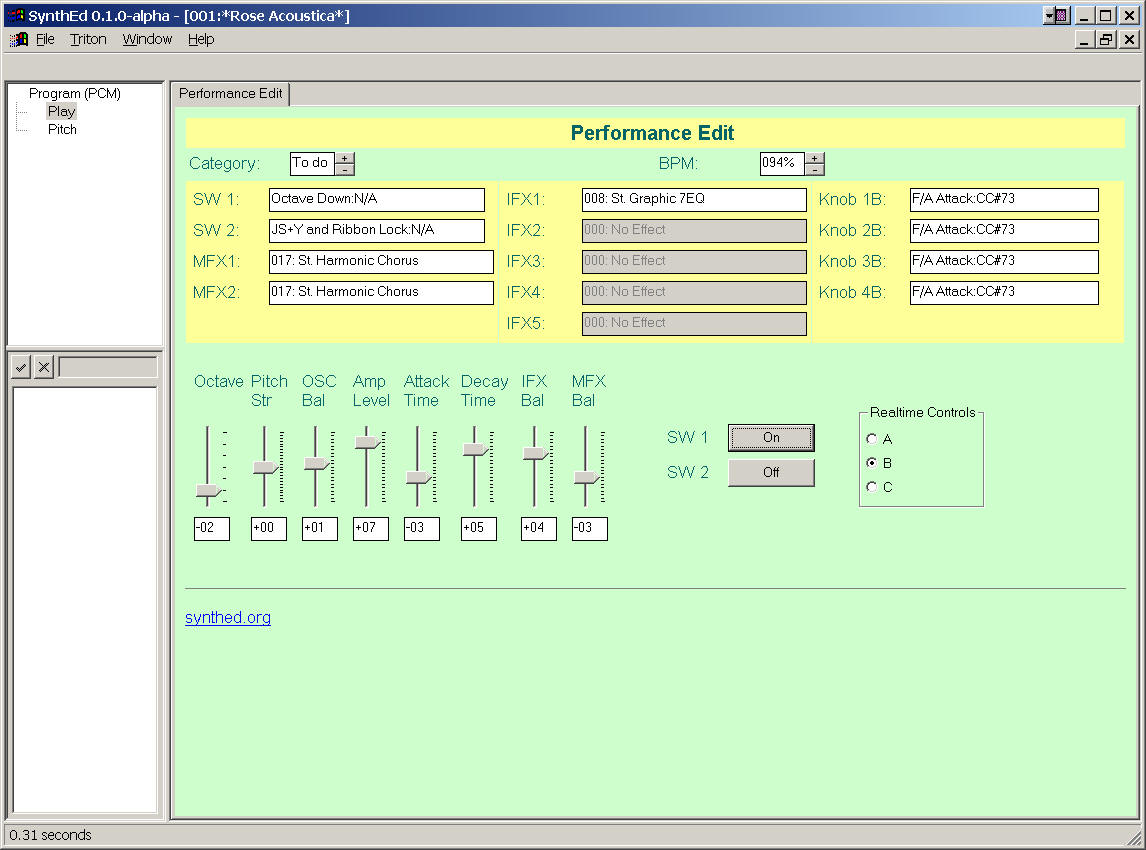
\includegraphics[scale=0.15]{html_ui.jpg}
\caption{SynthEd Screen shot}
\end{figure}

Here is an excerpt of the example interface file for the
Korg TRITON family: \\
\begin{verbatim}
<?xml version="1.0"?>
<!-- - - - - - - - - - - - - - - - - - - - - - - - - - - - - - -
    triton_ui.xml
- - - - - - - - - - - - - - - - - - - - - - - - - - - - - - - -->

<!DOCTYPE interface SYSTEM "../../interface.dtd">

<interface id="triton" caption="TRITON">

<!-- - - - - - - - - - - - - - - - - - - - - - - - - - - - - - - -
    Each editable mode is described here.
- - - - - - - - - - - - - - - - - - - - - - - - - - - - - - - -->
<modes>

<!-- - - - - - - - - - - - - - - - - - - - - - - - - - - - - - -
    Program mode.
 - - - - - - - - - - - - - - - - - - - - - - - - - - - - - - -->
<mode id="pcm" patch="pcm" caption="Program (PCM)">
    <page caption="Play">
        <tab caption="Performance Edit" url="triton_perfedit.htm"/>
        <tab caption="Arpeggiator" url="triton_arp.htm"/>
    </page>
    <page caption="Edit-Basic">
        <tab caption="Program Basic" url="triton_pgmbasic.htm"/>
        <tab caption="OSC Basic" url="triton_oscbasic.htm"/>
    </page>
    <page caption="Pitch">
        <tab caption="Pitch EG" url="triton_pitcheg.htm"/>
    </page>
</mode>

</modes>
</interface>
\end{verbatim}

\subsection{$<$mode$>$}
The \code{<mode>}{} element associates a patch with a set of
editor pages.
\\
\\
\\
\begin{tabular}{|l|c|p{9cm}|}
\hline
Attribute & Required & Description \\
\code{id} & Y & a unique name for the mode. \\
\code{patch} & Y & That patch type that is edited by this mode.
The value must match the id of a \code{<patch>}{} element in a patch file. \\
\code{caption} & N & The caption that SynthEd will display
in the window title bar. \\
\hline
\end{tabular}

\subsection{$<$page$>$} The \code{<page>}{} element groups
together a set of tabs (editor pages).
\\
\\
\\
\begin{tabular}{|l|c|p{9cm}|}
\hline
Attribute & Required & Description \\
\code{caption} & N & The caption that SynthEd will display in
the tree control. \\
\hline
\end{tabular}

\subsection{$<$tab$>$}
The \code{<tab>}{} element defines the location of an HTML edit
page.
\\
\\
\\
\begin{tabular}{|l|c|p{9cm}|}
\hline
Attribute & Required & Description \\
\code{caption} & N & The caption that SynthEd will display as
the tab label. \\
\code{url} & Y & location of an HTML edit page.  Relative paths
are evaluated relative
to the path of the interface file. \\
\code{mode} & N & Refer to the section on Dynamic
Content. \ref{dynamic_content} \\
\code{decoder} & N & Refer to the section on
Dynamic Content. \ref{dynamic_content} \\
\code{reset} & N & Refer to the section on
Dynamic Content. \ref{dynamic_content} \\
\hline
\end{tabular}

\section{Editor Files}\label{edit_files}
The basic unit of a SynthEd editor is an editor. Each editor is an
HTML document that positions widgets to permit synth parameter
editing. The HTML document displays when the user clicks on the
corresponding tab. Here is an excerpt of a sample editor:

\begin{verbatim}
<!DOCTYPE HTML PUBLIC "-//SoftQuad Software//DTD HoTMetaL PRO
6.0::19990601::extensions to HTML 4.0//EN" "hmpro6.dtd">
<HTML>
  <HEAD>
     <TITLE>Performance Edit</TITLE>
  </HEAD>
  <BODY BGCOLOR="#CCFFCC">
     <TABLE CELLSPACING="1">
        <TR>
          <TD WIDTH="100"><FONT COLOR="#006666"
            FACE="Arial">Category:</FONT></TD>
          <TD>
             <WIDGET CLASS="ChoiceWidget" DECODER="list_categories">
                <PARAMETER ID="COMMON_category"></PARAMETER>
             </WIDGET> </TD>
          <TD WIDTH="60"><FONT COLOR="#006666"
            FACE="Arial">BPM:</FONT></TD>
          <TD>
             <WIDGET CLASS="SpinWidget" DECODER="scale_arp_gate">
                <PARAMETER ID="ARP_gate"></PARAMETER>
             </WIDGET> </TD>
        </TR>
     </TABLE>
     <TABLE BGCOLOR="#FFFF99" CELLSPACING="1">
        <TR>
          <TD VALIGN="TOP">
             <TABLE BGCOLOR="#FFFF99" CELLSPACING="1">
                <TR>
                  <TD WIDTH="60"><FONT COLOR="#006666"
                    FACE="Arial">SW 1:</FONT></TD>
                  <TD>
                     <WIDGET CLASS="TextWidget" DECODER="list"
                        REFERENCE="list_1-2">
                        <PARAMETER ID="COMMON_sw1_assign_type">
                        </PARAMETER>
                     </WIDGET> </TD>
                </TR>
                <TR>
                  <TD><FONT COLOR="#006666"
                     FACE="Arial">SW 2:</FONT></TD>
                  <TD>
                     <WIDGET CLASS="TextWidget" DECODER="list_1-2">
                        <PARAMETER ID="COMMON_sw2_assign_type">
                        </PARAMETER>
                     </WIDGET> </TD>
                </TR>
                <TR>
                  <TD><FONT COLOR="#006666"
                     FACE="Arial">MFX1:</FONT></TD>
                  <TD>
                     <WIDGET CLASS="TextWidget"
                        DECODER="list_effects_single">
                        <PARAMETER ID="MFX1_effect_no"></PARAMETER>
                     </WIDGET> </TD>
                </TR>
                <TR>
                  <TD><FONT COLOR="#006666"
                     FACE="Arial">MFX2:</FONT></TD>
                  <TD>
                     <WIDGET CLASS="TextWidget"
                        DECODER="list_effects_single">
                        <PARAMETER ID="MFX1_effect_no"></PARAMETER>
                     </WIDGET> </TD>
                </TR>
             </TABLE> </TD>
          <TD>
        </TR>
     </TABLE>
  </BODY>
</HTML>
\end{verbatim}

SynthEd supports a subset of HTML tags. SynthEd's HTML
implementation uses the
\hlink{wxWindows}{http://www.wxwindows.org} library, from which
the following list of supported HTML elements and attributes is
derived. The following tables list all HTML elements known to
SynthEd, together with their supported attributes. An element
takes the general form of \\
 {\tt <tagname attribute\_1 attribute\_2 ... attribute\_n>} \\
 where attribute\_i is {\tt attributename="attributevalue"}.
Unless stated otherwise, SynthEd HTML is case-insensitive.

\subsection{Supported HTML Elements}

\begin{verbatim}

A               NAME=[string]
                HREF=[url]
                TARGET=[target window spec]
ADDRESS
AREA            SHAPE=POLY
                SHAPE=CIRCLE
                SHAPE=RECT
                COORDS=[coords]
                HREF=[url]
B
BIG
BLOCKQUOTE
BODY            TEXT=[color]
                LINK=[color]
                BGCOLOR=[color]
BR              ALIGN=[alignment]
CENTER
CITE
CODE
DD
DIV             ALIGN=[alignment]
DL
DT
EM
FONT            COLOR=[color]
                SIZE=[fontsize]
                FACE=[comma-separated list of facenames]
HR              ALIGN=[alignment]
                SIZE=[pixels]
                WIDTH=[percent|pixels]
                NOSHADE
H1
H2
H3
H4
H5
H6
I
IMG             SRC=[url]
                WIDTH=[pixels]
                HEIGHT=[pixels]
                ALIGN=TEXTTOP
                ALIGN=CENTER
                ALIGN=ABSCENTER
                ALIGN=BOTTOM
                USEMAP=[url]
KBD
LI
MAP             NAME=[string]
META            HTTP-EQUIV="Content-Type"
                CONTENT=[string]
OL
P               ALIGN=[alignment]
PRE
SAMP
SMALL
STRIKE
STRONG
TABLE           ALIGN=[alignment]
                WIDTH=[percent|pixels]
                BORDER=[pixels]
                VALIGN=[v_alignment]
                BGCOLOR=[color]
                CELLSPACING=[pixels]
                CELLPADDING=[pixels]
TD              ALIGN=[alignment]
                VALIGN=[v_alignment]
                BGCOLOR=[color]
                WIDTH=[percent|pixels]
                COLSPAN=[pixels]
                ROWSPAN=[pixels]
TH              ALIGN=[alignment]
                VALIGN=[v_alignment]
                BGCOLOR=[color]
                WIDTH=[percent|pixels]
                COLSPAN=[pixels]
                ROWSPAN=[pixels]
TITLE
TR              ALIGN=[alignment]
                VALIGN=[v_alignment]
                BGCOLOR=[color]
TT
U
UL

\end{verbatim}

\subsection{Supported HTML Attributes}

SynthEd will use the following HTML attributes:

\begin{verbatim}
[alignment]     CENTER
                LEFT
                RIGHT
                JUSTIFY

[v_alignment]   TOP
                BOTTOM
                CENTER

[color]         HTML 4.0-compliant color specification

[fontsize]      -2
                -1
                +0
                +1
                +2
                +3
                +4
                 1
                 2
                 3
                 4
                 5
                 6
                 7

[pixels]        integer value that represents dimension in pixels

[percent]       i%
                where i is integer

[url]           an URL

[string]        text string

[coords]        c(1),c(2),c(3),...,c(n)
                where c(i) is integer

\end{verbatim}

In addition to these standard HTML tags, SynthEd supports a set of
extended HTML tags.

\subsection{Extended HTML tags} SynthEd extends HTML with custom
tags to define widgets to edit synth parameters:
\subsubsection{$<$widget$>$}

The \code{<widget>}{} element constructs a widget to edit one or
more synth parameters.
\\
\\
\\
\begin{tabular}{|l|c|p{9cm}|}
\hline
Attribute & Required & Description \\
\code{class} & Y & The case-sensitive name of a widget class. \\
\code{width} & N & Width in pixels or percent; default = ``100\%'' \\
\code{decoder} & N & The id of a decoder. \\
\code{enable} & N & A Python expression that sets the
enabled state of the widget. \\
\hline
\end{tabular}
\\
\\
\\
If a \code{width}{} is specified in pixels, then the display width
of the widget is fixed at the specified number of pixels. If the
\code{width}{} is specified as a percentage, then the display
width of the widget will be adjusted to use the specified
percentage of the width of its container. Placing a widget in a
table with a percentage width allows the widget's width to adjust
dynamically with the table.

If an \code{enable}{} attribute is specified, the widget will be
enabled at runtime if the attribute value evaluates to non-zero;
the widget will be disabled at runtime if the attribute value
evaluates to zero. If a parameter is referenced by the
\code{enable}{} attribute, you will usually want to also include
the parameter as a child parameter to the widget. This will
register the widget with the referenced parameter, so that the
enable state of the widget will automatically update if the
referenced parameter value changes. For example:

\begin{verbatim}
    <WIDGET CLASS="ChoiceWidget" DECODER="list_multisamples"
        enable="COMMON_osc_mode.getData() == 2">
        <PARAMETER ID="COMMON_osc_mode" indexer="false"></PARAMETER>
        <PARAMETER ID="COMMON_bank_no"></PARAMETER>
        <PARAMETER ID="COMMON_multisample_no"></PARAMETER>
    </WIDGET>
\end{verbatim}

The widget in this example will be enabled only if the
\code{COMMON\_osc\_mode}{} parameter value equals \code{2}. The
\code{COMMON\_osc\_mode}{} also appears in the parameter list, so
that the \code{enable}{} expression will be re-evaluated if the
oscillator mode is changed by another widget. Since the
\code{indexer}{} attribute is false, the oscillator mode will not
be used to compute the display value for the widget.
\\
\\
\\
The following widget classes are implemented:
\\
\\
\\
\begin{tabular}{|l|p{9cm}|}
\hline
Class & Description \\
\hline
\code{ButtonWidget} & A push button. \\
\code{CheckWidget} & A check box. \\
\code{ChoiceWidget} & A drop-down combo box. \\
\code{EditWidget} & An editable text box. \\
\code{EnvelopeWidget} & A graphical envelope control. \\
\code{GaugeWidget} & A gauge. \\
\code{LabelWidget} & A text label. \\
\code{RadioWidget} & A radio box. \\
\code{SliderWidget} & A slider control. \\
\code{SpinWidget} & A spinner control. \\
\code{TextWidget} & A non-editable text box. \\
\code{Group} & A group of widgets. \\
\code{-} & Any custom widgets as developed. \\
\hline
\end{tabular}

\subsubsection{$<$parameter$>$}
A \code{<widget>}{} may contain zero or more \code{<parameter>}{}
elements.
\\
\\
\\
\begin{tabular}{|l|c|p{9cm}|}
\hline
Attribute & Required & Description \\
\code{id} & Y & The id of the referenced parameter. \\
\code{indexer} & N & Is this value a list index? [true$|$false] \\
\hline
\end{tabular}
\\
\\
\\
Each \code{<parameter>}{} element that appears in an edit page is
a reference to a parameter in a patch. One parameter may be
referenced by more than one widget. When SynthEd instantiates a
widget, the widget is registered with each of its child
parameters. If a given parameter value is set or changed by any
one widget, all other registered widgets are automatically
refreshed to reflect the new parameter value.

While one widget may reference many parameters, most widgets only
set (update) the {\it last} parameter value. If more than one
parameter is included in such a widget, only the last parameter is
updated. For example two parameters are specified in the following
example:

\begin{verbatim}
    <WIDGET CLASS="ChoiceWidget" DECODER="list_multisamples">
        <PARAMETER ID="COMMON_bank_no"></PARAMETER>
        <PARAMETER ID="COMMON_multisample_no"></PARAMETER>
    </WIDGET>
\end{verbatim}

While the ChoiceWidget will be refreshed if either
\code{COMMON\_bank\_no}{} or \code{COMMON\_multisample\_no}{}
parameter values change, only the {\it last} parameter value,
\code{COMMON\_multisample\_no}{}, will be set if the user selects
a new value from the ChoiceWidget's combo box.

\subsection{Widgets}
Each of the standard SynthEd widgets is presented.

\subsubsection{ButtonWidget}
A \code{ButtonWidget}{} is a push-button widget. Each time the
widget is clicked (pressed), it increments its parameter value by
1. If the new parameter value exceeds the max parameter value, the
parameter value is set to the min parameter value. The face of the
push-button displays the current display value of the parameter.
\\
\\
\\
\begin{tabular}{|l|c|p{9cm}|}
\hline
Attribute & Required & Description \\
\code{class} & Y & The case-sensitive name of a widget class. \\
\code{width} & N & Width in pixels or percent; default = ``100\%'' \\
\code{decoder} & N & The id of a decoder. \\
\code{enable} & N & A Python expression that sets the
enabled state of the widget. \\
\code{tip} & N & This text will be displayed in a tool tip. \\
\hline
\end{tabular}

\subsubsection{CheckWidget}
A \code{CheckWidget}{} is a check-box widget. Clicking the widget
toggles the checked state of the check-box. If the check-box is
checked, the parameter value is set to \code{1}{}; if the box is
unchecked, the parameter value is set to \code{0}{}.
\\
\\
\\
\begin{tabular}{|l|c|p{9cm}|}
\hline
Attribute & Required & Description \\
\code{class} & Y & The case-sensitive name of a widget class. \\
\code{width} & N & Width in pixels or percent; default = ``100\%'' \\
\code{decoder} & N & The id of a decoder. \\
\code{enable} & N & A Python expression that sets the
enabled state of the widget. \\
\code{tip} & N & This text will be displayed in a tool tip. \\
\hline
\end{tabular}

\subsubsection{ChoiceWidget}
A \code{ChoiceWidget}{} is a drop-down combo box widget. Clicking
the combo-box will drop down a list of available items. Selecting
an item will set the parameter value to the index of the selected
item.
\\
\\
\\
\begin{tabular}{|l|c|p{9cm}|}
\hline
Attribute & Required & Description \\
\code{class} & Y & The case-sensitive name of a widget class. \\
\code{width} & N & Width in pixels or percent; default = ``100\%'' \\
\code{decoder} & N & The id of a decoder. \\
\code{enable} & N & A Python expression that sets the
enabled state of the widget. \\
\code{tip} & N & This text will be displayed in a tool tip. \\
\hline
\end{tabular}

\subsubsection{EditWidget}
A \code{EditWidget}{} is an editable text box widget that is
normally used to edit a string parameter value.
\\
\\
\\
\begin{tabular}{|l|c|p{9cm}|}
\hline
Attribute & Required & Description \\
\code{class} & Y & The case-sensitive name of a widget class. \\
\code{width} & N & Width in pixels or percent; default = ``100\%'' \\
\code{decoder} & N & The id of a decoder. \\
\code{enable} & N & A Python expression that sets the
enabled state of the widget. \\
\code{tip} & N & This text will be displayed in a tool tip. \\
\hline
\end{tabular}

\subsubsection{EnvelopeWidget}
A \code{EnvelopeWidget}{} is a graphical depiction of an envelope.
The envelope maps a set of parameter values to points in an (x,y)
coordinate plane. For example:
\\
\\
\\
\begin{tabular}{|l|c|p{9cm}|}
\hline
Attribute & Required & Description \\
\code{class} & Y & The case-sensitive name of a widget class. \\
\code{width} & N & Width in pixels or percent; default = ``100\%'' \\
\code{decoder} & N & The id of a decoder. \\
\code{enable} & N & A Python expression that sets the
enabled state of the widget. \\
\code{tip} & N & This text will be displayed in a tool tip. \\
\hline
\end{tabular}
\\
\\
\\

\begin{verbatim}
    <WIDGET CLASS="EnvelopeWidget">
        <PARAMETER ID="CONSTANT_0"></PARAMETER>
        <PARAMETER ID="PITCH_EG_start_level"></PARAMETER>
        <PARAMETER ID="PITCH_EG_attack_time"></PARAMETER>
        <PARAMETER ID="PITCH_EG_attack_level"></PARAMETER>
        <PARAMETER ID="PITCH_EG_decay_time"></PARAMETER>
        <PARAMETER ID="CONSTANT_0"></PARAMETER>
        <PARAMETER ID="PITCH_EG_release_time"></PARAMETER>
        <PARAMETER ID="PITCH_EG_release_level"></PARAMETER>
    </WIDGET>
\end{verbatim}

The example envelope consists of 4 points:
\\
\\
\\
\begin{tabular}{|r|l|l|}
\hline
Point & X & Y \\
\hline
1 & CONSTANT\_0 & PITCH\_EG\_start\_level \\
2 & PITCH\_EG\_attack\_time & PITCH\_EG\_attack\_level \\
3 & PITCH\_EG\_decay\_time & CONSTANT\_0 \\
4 & PITCH\_EG\_release\_time & PITCH\_EG\_release\_level \\
\hline
\end{tabular}
\\
\\
\\
Generally, the X component is a {\it time} parameter and the Y
component is a {\it level} parameter. The \code{EnvelopeWidget}{} is
somewhat unique in that it can set (update) the values of multiple
parameters.

\subsubsection{GaugeWidget}
A \code{GaugeWidget}{} is a widget that displays a horizontal or
vertical gauge with a start and stop value.
\\
\\
\\
\begin{tabular}{|l|c|p{9cm}|}
\hline
Attribute & Required & Description \\
\code{class} & Y & The case-sensitive name of a widget class. \\
\code{width} & N & Width in pixels or percent; default = ``100\%'' \\
\code{layout} & N & Orientation [horizontal$|$vertical] \\
\code{decoder} & N & The id of a decoder. \\
\code{enable} & N & A Python expression that sets the
enabled state of the widget. \\
\code{tip} & N & This text will be displayed in a tool tip. \\
\hline
\end{tabular}

\subsubsection{LabelWidget}
A \code{LabelWidget}{} is a widget that displays a label.
\\
\\
\\
\begin{tabular}{|l|c|p{9cm}|}
\hline
Attribute & Required & Description \\
\code{class} & Y & The case-sensitive name of a widget class. \\
\code{width} & N & Width in pixels or percent; default = ``100\%'' \\
\code{decoder} & N & The id of a decoder. \\
\code{enable} & N & A Python expression that sets the
enabled state of the widget. \\
\code{tip} & N & This text will be displayed in a tool tip. \\
\hline
\end{tabular}

\subsubsection{RadioWidget}
A \code{RadioWidget}{} is a widget that displays a radio box.
\\
\\
\\
\begin{tabular}{|l|c|p{9cm}|}
\hline
Attribute & Required & Description \\
\code{class} & Y & The case-sensitive name of a widget class. \\
\code{width} & N & Width in pixels or percent; default = ``100\%'' \\
\code{layout} & N & Orientation [horizontal$|$vertical] \\
\code{decoder} & N & The id of a decoder. \\
\code{enable} & N & A Python expression that sets the
enabled state of the widget. \\
\code{tip} & N & This text will be displayed in a tool tip. \\
\hline
\end{tabular}

\subsubsection{SliderWidget}
A \code{SliderWidget}{} is a widget that displays a slider and an
attached edit box. The managed parameter value may be adjusted
either by moving the slider or by entering a value in the edit
box.
\\
\\
\\
\begin{tabular}{|l|c|p{9cm}|}
\hline
Attribute & Required & Description \\
\code{class} & Y & The case-sensitive name of a widget class. \\
\code{width} & N & Width in pixels or percent; default = ``100\%'' \\
\code{layout} & N & Orientation [horizontal$|$vertical] \\
\code{decoder} & N & The id of a decoder. \\
\code{enable} & N & A Python expression that sets the
enabled state of the widget. \\
\code{tip} & N & This text will be displayed in a tool tip. \\
\hline
\end{tabular}

\subsubsection{SpinWidget}
A \code{SpinWidget}{} is a widget that displays a spinner and an
attached edit box. The managed parameter value may be adjusted
either by clicking the spinner buttons or by entering a value in
the edit box.
\\
\\
\\
\begin{tabular}{|l|c|p{9cm}|}
\hline
Attribute & Required & Description \\
\code{class} & Y & The case-sensitive name of a widget class. \\
\code{width} & N & Width in pixels or percent; default = ``100\%'' \\
\code{layout} & N & Orientation [horizontal$|$vertical] \\
\code{decoder} & N & The id of a decoder. \\
\code{enable} & N & A Python expression that sets the
enabled state of the widget. \\
\code{tip} & N & This text will be displayed in a tool tip. \\
\hline
\end{tabular}

\subsubsection{TextWidget}
A \code{TextWidget}{} is an non-editable text box widget.
\\
\\
\\
\begin{tabular}{|l|c|p{9cm}|}
\hline
Attribute & Required & Description \\
\code{class} & Y & The case-sensitive name of a widget class. \\
\code{width} & N & Width in pixels or percent; default = ``100\%'' \\
\code{decoder} & N & The decoder type [list$|$scale]. \\
\code{enable} & N & A Python expression that sets the enabled
state of the widget. \\
\code{tip} & N & This text will be displayed in a tool tip. \\
\hline
\end{tabular}

\subsubsection{GroupWidget}
A \code{GroupWidget}{} does not itself display, but manages a
group of widgets. It serves to enable/disable a group of widgets.
\\
\\
\\
\begin{tabular}{|l|c|p{9cm}|}
\hline
Attribute & Required & Description \\
\code{class} & Y & The case-sensitive name of a widget class. \\
\code{enable} & N & A Python expression that sets the enabled
state of the widget. \\
\hline
\end{tabular}
\\
\\
\\
The \code{GroupWidget}{} is unique in that it can contain child
\code{<widget>}{} elements.

 For example:
\begin{verbatim}
    <WIDGET CLASS="GroupWidget"
        enable="COMMON_osc_mode.getData() == 2">
        <PARAMETER ID="COMMON_osc_mode" indexer="false"></PARAMETER>
        <WIDGET CLASS="SliderWidget"> ... </WIDGET>
        <WIDGET CLASS="SliderWidget"> ... </WIDGET>
        <WIDGET CLASS="SliderWidget"> ... </WIDGET>
        <WIDGET CLASS="SliderWidget"> ... </WIDGET>
    </WIDGET>
\end{verbatim}

The \code{GroupWidget}{} enables or disables all child widgets
based on its \code{enable}{} attribute. Use the
\code{GroupWidget}{} to avoid having to repeat the same
\code{enable}{} attribute for many different widgets.

\section{Dynamic Content}\label{dynamic_content}

Sometimes the meaning of a synth data object may change depending
upon certain factors. For example, in the Korg Triton family of
synths, a program may use up to 5 insert effects and up to two
master effects, choosing from a palette of 102 different effects
algorithms, each with its own unique set of parameters. To deal
with this, SynthEd provides a data-driven mechanism in the
interface file to dynamically reinterpret data objects and select
matching tabs (editors):

\begin{verbatim}
<?xml version="1.0"?>
<!DOCTYPE interface SYSTEM "../../interface.dtd">

<interface id="triton" caption="TRITON"> <modes>

<!-- - - - - - - - - - - - - - - - - - - - - - - - - - - -  - - -
    Program mode.
- - - - - - - - - - - - - - - - - - - - - - - - - - - - - - - -->
<mode id="pcm" patch="pcm" caption="Program (PCM)">
   <page caption="Insert Effect">
      <tab caption="Routing" url="triton_routing.htm"/>
      <tab caption="Insert FX" url="triton_insertfx.htm"/>
      <!-- The mode attribute indicates dynamic content.-->
      <tab caption="IFX 1" mode="fx" decoder="scale_fx_tabs"
        reset="true">
          <parameter id="IFX1_data_offset"/>
          <parameter id="IFX1_effect_no"/>
      </tab>
      <tab caption="IFX 2" mode="fx" decoder="scale_fx_tabs"
        reset="true">
          <parameter id="IFX2_data_offset"/>
          <parameter id="IFX2_effect_no"/>
      </tab>
      <tab caption="IFX 3" mode="fx" decoder="scale_fx_tabs"
        reset="true">
          <parameter id="IFX3_data_offset"/>
          <parameter id="IFX3_effect_no"/>
      </tab>
      <tab caption="IFX 4" mode="fx" decoder="scale_fx_tabs"
        reset="true">
          <parameter id="IFX4_data_offset"/>
          <parameter id="IFX4_effect_no"/>
      </tab>
      <tab caption="IFX 5" mode="fx" decoder="scale_fx_tabs"
        reset="true">
          <parameter id="IFX5_data_offset"/>
          <parameter id="IFX5_effect_no"/>
      </tab>
   </page>
</mode>

<mode id="fx" caption="Effects">
   <page caption="Effects Editors">
      <tab patch="fx_000" caption="No Effect"
         url="triton_fx000.htm"/>
      <tab patch="fx_001" caption="St.Amp Simulation"
         url="triton_fx001.htm"/>
      <tab patch="fx_002" caption="Stereo Compressor"
         url="triton_fx002.htm"/>
      <tab patch="fx_003" caption="Stereo Limiter"
         url="triton_fx003.htm"/>
      <tab patch="fx_004" caption="Multiband Limiter"
         url="triton_fx004.htm"/>
      <tab patch="fx_005" caption="Stereo Gate"
         url="triton_fx005.htm"/>
   </page>
</mode>

</modes>
</interface>
\end{verbatim}

\subsection{Dynamic $<$tab$>$ elements}

The following \code{<tab>}{} attributes are used for dynamic
editor switching:
\\
\\
\begin{tabular}{|l|c|p{9cm}|}
\hline
Attribute & Required & Description \\
\code{mode} & N & The mode containing the list of possible editors. \\
\code{decoder} & N & Decoder returning the patch id to use.  \\
\code{reset} & N & Should the parameters values be re-initialized
after a switch [true | false]. \\
\hline
\end{tabular}
\\
\\
\\
The \code{mode}{} attribute should match the id of a
\code{<mode>}{} element. In the example, the value \code{fx}{}
refers to the \code{<mode id="fx">}{} element defining the
available effects editors.

The \code{decoder}{} attribute should match the id of a decoder that
will accept as input a parameter data value and output a corresponding
patch name.

If \code{reset}{} is true, then SynthEd will re-initialize the
affected parameter values on a switch. For example, suppose that
the user switches from IFX (Insert Effect) algorithm 1 (Stereo Amp
Simulator) to IFX algorithm 2 (Stereo Compressor). During the
switch, the patch or data object may be reinterpreted, and
parameter values that may have been perfectly valid for algorithm
1, when reinterpreted, may produce illegal data values for
algorithm 2. The \code{reset}{} option will re-initialize the
parameters to algorithm defaults.

A dynamic \code{<tab>}{} element must contain two child
\code{<parameter>}{} elements. The first parameter holds the patch
offset of the start of the dynamic content. The second parameter
will be decoded as the name of the editor to be used. In the above
example, the first dynamic tab contains the parameters:

\begin{verbatim}
      <parameter id="IFX1_data_offset"/>
      <parameter id="IFX1_effect_no"/>
\end{verbatim}

which refer to the corresponding patch parameters in the example
Program (PCM) patch file \ref{patch_files}:

\begin{verbatim}
    ...

    <!-- Insert Effects -->
    <!-- IFX1_data_offset holds the patch offset of IFX1 -->
    <parameter id="IFX1_data_offset" min="16" max="16"/>
    <parameter id="IFX1_effect_no" min="0x00" max="0x59">
        <byte offset="32"/>
    </parameter>

    ...
\end{verbatim}

So in this example, \code{IFX1\_data\_offset}{} holds the offset
of the IFX1 (Insert Effect 1) data object in the Program (PCM)
patch and \code{IFX1\_effect\_no}{} holds an effect algorithm
number between 0 and 89.

The decoder attribute value \code{scale\_fx\_tabs}{} refers to the
corresponding decoder in the Triton decoder file
\ref{decoder_files}, which is excerpted here:

\begin{verbatim}

<!-- - - - - - - - - - - - - - - - - - - - - - - - - - - - - - -
    FX tabs
 - - - - - - - - - - - - - - - - - - - - - - - - - - - - - - -->

<scale id="scale_fx_tabs" min="0x00" max="0x66" format="fx_%03d">
    <range min="0x00" max="0x66" minval="0" increment="1"/>
</scale>
\end{verbatim}

This decoder will convert the \code{IFX1\_effect\_no}:
\begin{tabular}{|r|r|} \hline
Input Value & Output Value \\
\hline
0 & fx\_000 \\
1 & fx\_001 \\
2 & fx\_002 \\
3 & fx\_003 \\
... & ... \\
\hline
\end{tabular}
\\
\\
\\

\subsection{Dynamic Tab Operation}

Here's what happens when the parameter \code{IFX\_effect\_no}{}
value changes while editing a Program (PCM) patch:

\begin{enumerate}
\item The value of \code{IFX\_effect\_no}{} changes from
\code{1}{} to \code{2}{} (presumably from user editing).

\item The \code{IFX 1}{} tab is notified of a change to its
registered parameter, \code{IFX\_effect\_no}.

\item When the \code{IFX 1}{} tab is next displayed, the tab's
decoder decodes the \code{IFX\_effect\_no}{} value \code{2}{} into
\code{fx\_002}.

\item The patch definition \code{<patch id="fx\_002">}{} matching
the decoded value \code{fx\_002}{} is located.

 \item The patch definition \code{<patch
id="fx\_002"}{} is applied to the current patch (Program PCM) at
offset \code{16}{}, the offset specified in
\code{IFX1\_data\_offset}.

\item If \code{reset="true"}, the \code{fx\_002}{} patch
parameters are initialized.

\item The interface \code{<mode id="fx">}{} matching the
\code{mode="fx"}{} attribute is located. The contained \code{<tab
patch="fx\_002">}{} matching the decoded value \code{fx\_002}{} is
located.

\item The resulting Stereo Compressor tab (editor) is displayed.
\end{enumerate}

\end{document}
